\subsection{Experiment Interfaces}

\subsubsection{Mechanical Interfaces}
\label{sec:4.2.1}

%\colorbox{orange}{\parbox{\textwidth}{THIS SECTION WILL BE FINALISED WHEN AN UPDATED CAD MODEL AND INTERFACE DESIGN WILL BE AVAILABLE}}\\

The experiment mounting platform will be attached to the lower rails of the gondola.

% Discuss mounting safety


\begin{figure}[H]
    \centering
	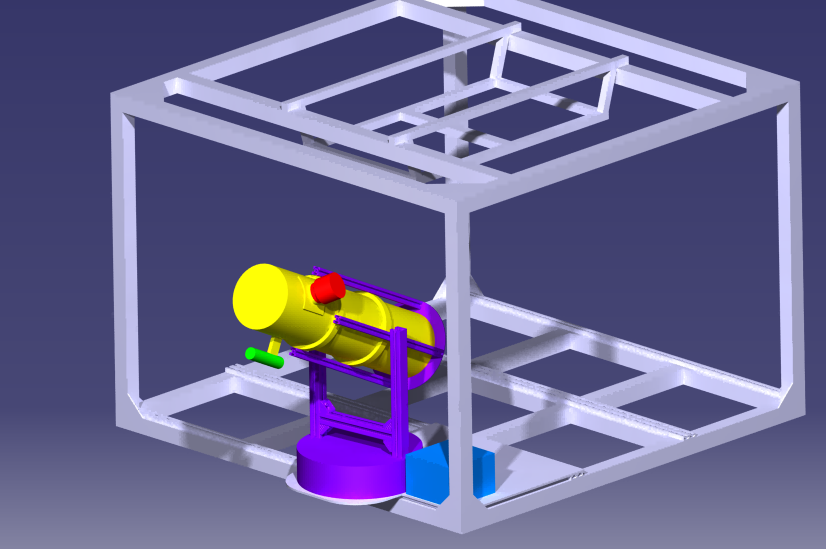
\includegraphics[width=0.9\linewidth]{4-experiment-design/img/mechanical/Assembly_v3iso2.png}
	\caption{Instrument position on gondola}
\end{figure}


% \bigskip
% \input{4-experiment-design/tables/attaching_comp.tex}


\subsubsection{Thermal Interfaces}

%\colorbox{orange}{\parbox{\textwidth}{THIS SECTION REQUIRES THERMAL ANALYSIS AND DESIGN}}\\

The IRISC experiment will be shielded from heat sources that could potentially introduce noise to the measurements. Once the final selection of components is made, Finite Element Analysis will be used to optimize the configuration of the components to ensure a good system performance.

\label{sec:4.2.2}


\subsubsection{Electrical Interfaces}
\label{sec:4.2.3}
\textbf{E-link:}\\
The uplink will be used to send occasional commands to control the experiment. One command will be [\hl{TBD}] in size. The TCP/IP protocol will be used for uplink, so the total size of one transmission will be the data plus the TCP header (maximum 480 bits), the IP header (maximum 480 bits) and the Ethernet frame (144 bits).

$$ bits\, per\, uplink\, packet \leq [TBD] + 480 + 480 + 144 $$

The downlink will be used to send science and housekeeping data to the ground station. The data in the downlink packet is estimated to be [\hl{TBD}]. For downlink, UDP protocol will be used, as the reliability of the data is not as crucial as during the uplink and to compensate for the size of the data packet. The total size of one packet will be the data plus the UDP header (32 bits), the IP header (maximum 480 bits) and the Ethernet frame (144 bits).

$$ bits\, per\, downlink\, packet \leq [TBD] + 32 + 480 + 144 $$

\textbf{Power:}\\

Placed on the outside of the experiment structure/housing, the experiment will have a 4 pin, male, box mount receptacle MIL–C-26482P series 1 connector with an 8-4 insert arrangement (MS3112E8-4P).


% I comment this out because of Tomas comment that poower in not an interface. Also removed the 1mA. 
% Power will be delivered to the electronics box from the provided 28.8 V (13 Ah) battery pack. Only one pack is required. The expected % minimum current is [\hl{TBD}], the average is [\hl{TBD}] and the maximum is [\hl{TBD}]. More details in \ref{sec:4.7}.

\textbf{Connectors:}\\

%\begin{figure}[H]
%    \centering
%	\includegraphics[width=0.2\linewidth]{4-experiment-design/img/interfaces/power_cables.jpg}
%	\caption{[\hl{PLACEHOLDER}] Position of power cable socket}
%	\label{fig:power_cables}
%\end{figure}
%
%\begin{figure}[H]
%    \centering
%	\includegraphics[width=0.2\linewidth]{4-experiment-design/img/interfaces/elink_cables.jpg}
%	\caption{[\hl{PLACEHOLDER}] Position of E-link cable socket}
%	\label{fig:elink_cables}
%\end{figure}

Info about power cables, their length/resistivity and thus power loss, their connection to gondola power relay.



\textbf{Connectors:}\\

\textbf{Protection:}\\

\textbf{Grounding:}\\


\subsubsection{Radio Frequencies (Optional)}



\raggedbottom
